% Demo presentation for the albatross template.
% Compile with: xelatex albatrossbeamer.tex

\documentclass{albatrossbeamer}

\title{Introduction to Meteorology}
\subtitle{A first look at the atmosphere}
\author{Author}
\date{\today}

\begin{document}

{ % background image scoped to the title slide only; swap this file for
  % a different presentation's own cover image
  \usebackgroundtemplate{%
    \begin{tikzpicture}[remember picture,overlay]
      \clip (current page.south west) rectangle (current page.north east);
      \node[opacity=1] at (current page.center)
        {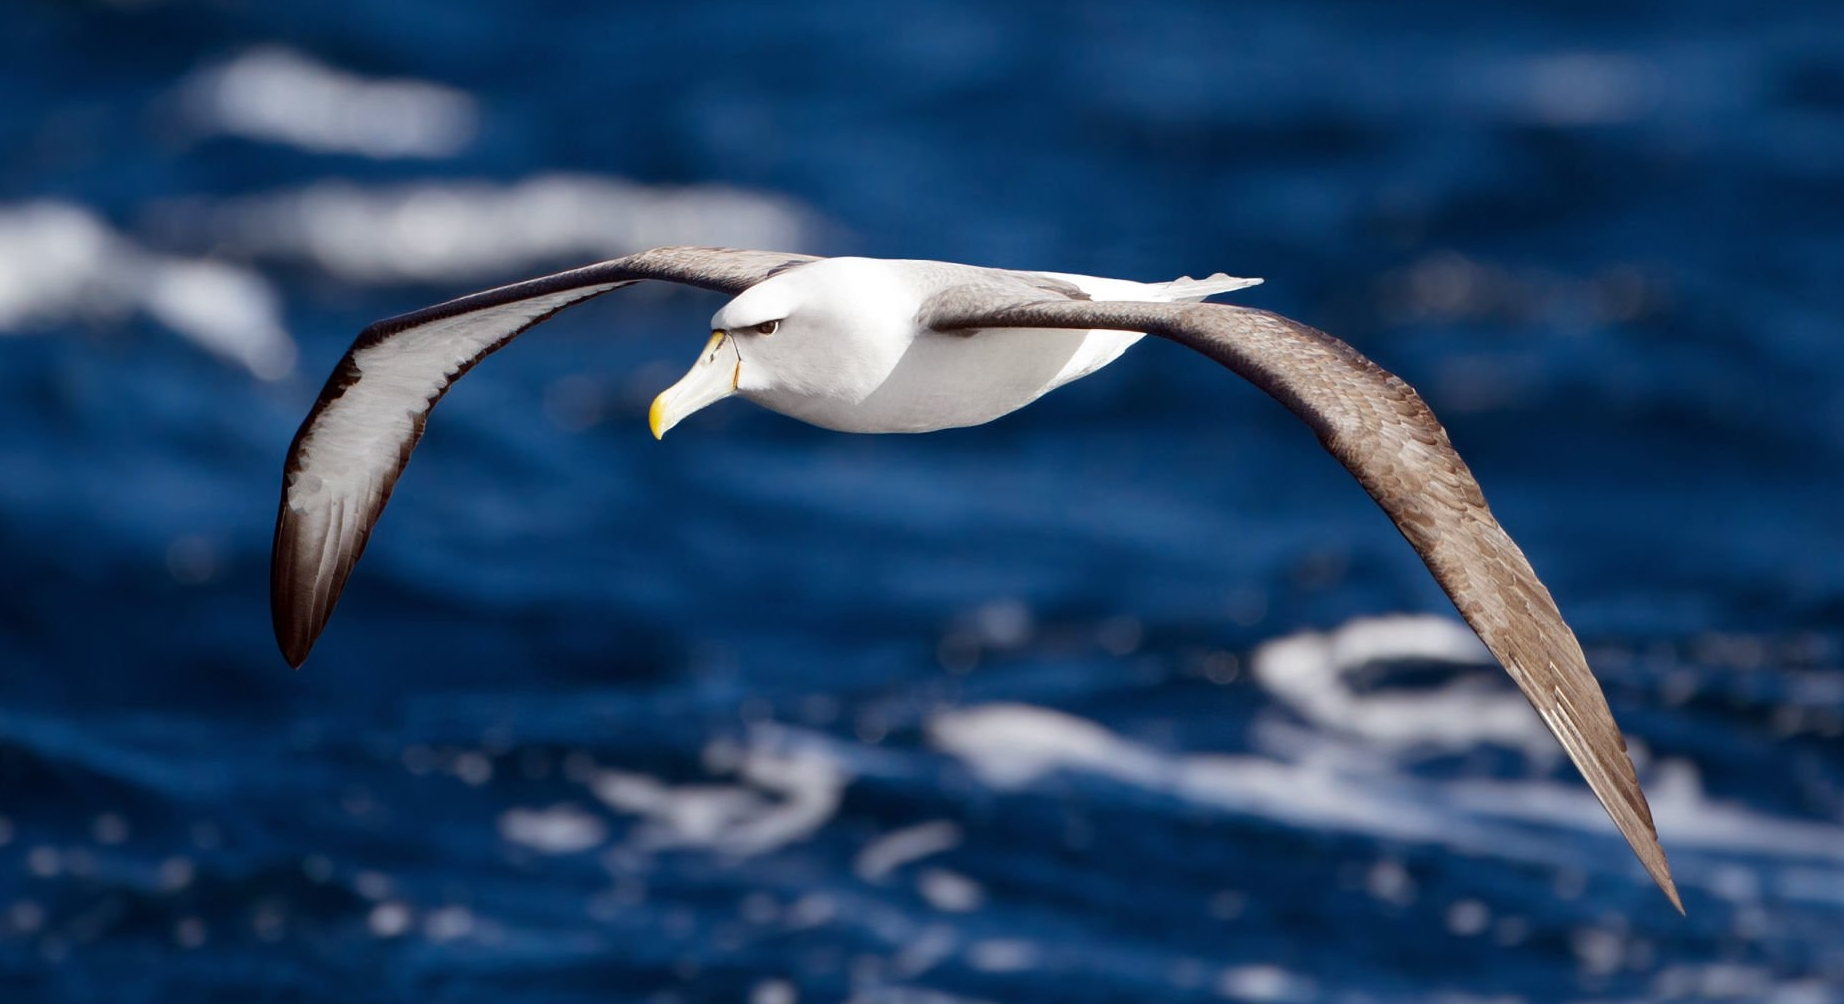
\includegraphics[height=\paperheight]{background/albatrosHD.jpg}};
    \end{tikzpicture}%
  }
  \begin{frame}[plain,noframenumbering]
    \maketitle
  \end{frame}
}

\begin{frame}{Writing a simple slide}
  \framesubtitle{Title, subtitle, body text}
  \begin{itemize}
    \item The slide title uses Bebas Neue in Deep Twilight
    \item The subtitle below it uses Lato in Bright Teal Blue
      \begin{itemize}
        \item Sub-bullets step down the sea palette to Bright Teal Blue
        \begin{itemize}
          \item And a third level continues to Turquoise Surf
        \end{itemize}
      \end{itemize}
    \item Body text uses Josefin Sans
    \item Use \alert{alert} to bring focus to something, in bold Deep Twilight
  \end{itemize}
\end{frame}

\begin{frame}{Content boxes}
  \framesubtitle{Two transparent box styles}
  \begin{columns}
    \column{.5\textwidth}
      \begin{seabox}{Seabox}
        Bright Teal Blue border, Light Cyan fill
      \end{seabox}
    \column{.5\textwidth}
      \begin{surfbox}
        Turquoise Surf border and fill
      \end{surfbox}
  \end{columns}
\end{frame}

\begin{frame}{Highlighting a region}
  \framesubtitle{Sunset accents for diagrams}
  \begin{center}
    \begin{tikzpicture}
      \node[anchor=south west,inner sep=0] (image) at (0,0)
        {
\includegraphics[width=0.5\textwidth]{logo/albatros-logo.png}};
      \begin{scope}[x={(image.south east)},y={(image.north west)}]
        \draw[sunsetorange,ultra thick,rounded corners] (0.55,0.3) rectangle (0.92,0.62);
        \draw[sunsetyellow,ultra thick] (0.22,0.55) circle (0.14);
      \end{scope}
    \end{tikzpicture}
  \end{center}
\end{frame}

\end{document}
